\section{Integer Programming}
\label{sec:ip}

Integer programming is just like linear programming, except we are only allowed
solutions inside $\mathbb{N}$ (the integers) instead of $\mathbb{R}$ (real
numbers). Even though we've narrowed our search space, the new problem turns out
to be harder (remember, even though our solutions will be finite and countable,
there are still a lot (very exponential) of them)!

We define \textit{mixed integer programming} to be linear programming, where
some variables are integers, but some are real numbers. Likewise, \textit{pure
integer programming} is when all the variables are integers.

At first, I thought integer programming was a bit pointless; couldn't you just
find the linear programming solution, and then round it down to the nearest
integer? Well, yes, but there are two issues; firstly, it might not be the best
solution, and secondly, you can do cool stuff with integer programming.

For example, what if we wanted to implement multiple choice? Say I want to buy
either car A, B, or C, and they all have safety ratings, prices, etc. I
obviously can't buy 0.375A, 0.005B and 0.62C; I have to make a decision.

We can encapsulate this in integer programming by having a constraint like this:

\[
  A + B + C \leq 1
\]

Furthermore, we can restrict variables to be binary too, which, if all our
variables are binary, actually turns out to be our old friend the knapsack
problem!

In fact, any pure integer programming problem can be expressed as a 0-1 problem,
since we can express any decimal number as a binary number.

\marginpar{We can also turn scheduling problems such as timetabling or the 
travelling salesman problem into integer programming problems.}

You may have worked out by this (if you remember the lectures from the second
half of this course, or if you have read later sections of this document), that
if we can turn the 0-1 knapsack problem into an integer programming problem,
then integer programming must be in the same complexity class as the knapsack
problem; meaning that integer programming is NP hard!

\subsection{Solving Integer Programming Problems}

It turns out, that \textit{Branch and Bound} is a good way to solve these kinds
of problems. If you remember the second year algorithms course, then you might
be having a quiet little groan right now. However, I have good news! There's a
really good explanation of B\&B in the course reading (the Chapter 9 handout you
should have picked up in the lecture).

Though it's good, and thorough, it's also a bit boring and dense. Here's my
shorter version, broken up into steps:

\begin{enumerate}
  \item So, we have an optimisation problem just like normal. We can graph it, 
  and it'll look something like this:

  \begin{figure}[H]
    \centering
    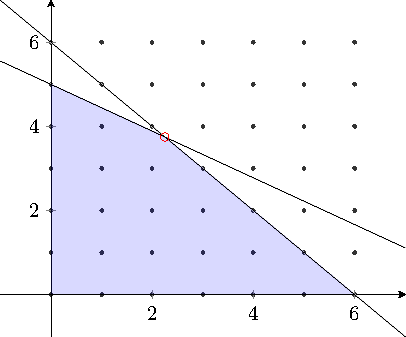
\includegraphics{diagrams/graph5}
    \caption{A graph of $y = 6 - x$, $y = \frac{45 - 5x}{9}$ and $x \geq 0,
      y \geq 0$. The linear optimum is shown as the red circle.}
    \label{fig:graph-5}
  \end{figure}

  This of course is a graph of two constraints relating to a maximisation
  problem. The problem and constraints are here:

  \[
    \begin{split}
      f = 5x + 8y\\
      x + y \leq 6\\
      5x + 9y \leq 45
    \end{split}
  \]

  If we use Simplex to solve this like a linear programming problem, then we get
  the optimum as $f(\frac{9}{4}, \frac{15}{4}) = 41.25$, which is obviously not
  a integral solution (since it has fractions).

  One thing to do might be to round off the numbers, trying $(2,4)$, which is
  infeasible due to the constraints and $2,3$ which gives $f=34$. However, while
  the latter solution is feasible, it is \textit{not} the optimum.

  \textbf{Note, in an example like this, you could enumerate all the integral 
  points and find which one is best. This was mentioned in the lectures and is 
  a lot easier than doing Branch and Bound!}

  \item If we don't have time to enumerate the points, then we need to do 
  branch and bound. We make use of the following observations:
  
  \begin{itemize}
    \item The integral solution isn't the same as the linear one for this
      problem, since the linear solution is not integral.
    \item The linear solution provides an upper bound on the integral solution.
  \end{itemize}

  In order to progress, you split the feasible region into half, along where
  either the $x$ or $y$ axis is equal to the linear optimum. We could split at
  $x = \frac{9}{4}$ or $y = \frac{15}{4}$, and will do the latter. Since our
  solutions are integral, we can discard the area between $3 < y < 4$:

  \begin{figure}[H]
    \centering
    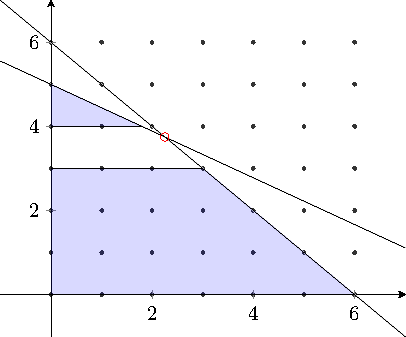
\includegraphics{diagrams/graph6}
    \caption{Now, we're showing the two feasible regions after we've split 
      along $y = \frac{15}{4}$}
    \label{fig:graph-6}
  \end{figure}

  Now, we have two problems; finding the integral solution to the upper region,
  and the lower region. Then we can simply pick the maximum!

\item To find the integral solution to each sub-region, simply add a new 
  constraint for each; for the top one, we add $y \geq 4$, and for the bottom 
  one, we add $y \leq 3$. Then we recurse to step 1 on both problems.

  However, because I'm nice, I'm going to do the recursion for you here:

  \begin{description}

  \item \textit{Top recursion}\\
  If we do this, we find that the linear solution for the top problem is
  $(\frac{9}{5}, 4)$, where $f = 41$. This isn't an integral, but we have gained
  important information; we can split the top area into two:

  \begin{figure}[H]
    \centering
    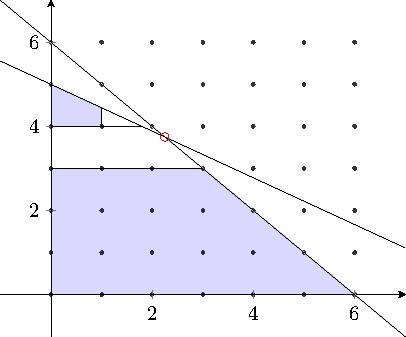
\includegraphics{diagrams/graph7}
    \caption{I've split the top area into two new areas where $x \leq 1$ and
    $x \geq 2$. Ohh wait, there aren't any integral points inside that last 
    one, so it's not shaded :)}
    \label{fig:graph-7}
  \end{figure}

  If we recurse again, we will find that the top part \textit{still} doesn't
  have an integral solution, but another level of recursion gives us two
  integral solutions (this is obvious if you think about it, since we can't
  recurse any more times due to the number of possible integer points inside the
  region); $f(1,4) = 37$, and $f(0,5) = 40$.

  \item \textit{Bottom recursion}\\
  If we recurse on the bottom region, and to simplex on it, we get an integral
  solution straight away; $f(3,3) = 39$. Since we know that the linear solution
  is an upper bound on the integral solution (hence we won't find a larger
  answer inside the rest of the lower region), then we can stop here.
  \end{description}

  Since the top region's result $f(0,5) = 40$ was better than the bottom
  region's one $f(3,3) = 39$, and those regions had inside them all the
  feasible points, then we have found our solution, $f(0,5) = 40$.

  If you understood all that, then I recommend you read Chapter 9 of the course
  handout (from section 9.4 on page 287 to the end of section 9.5 on page 292),
  since it visualises the above as a tree as well. Besides, you've already
  understood the concept, so it'll be light reading!

\end{enumerate}
